\chapter{Introduzione Ambiente distribuito}

L'universo in cui opereremo sarà chiamato \textbf{ambiente di calcolo
    distribuito}. È costituito da un insieme finito $\epsilon$ di \textbf{entità}
computazionali che comunicano per mezzo di \textbf{messaggi}. Le entità
comunicano con altre entità per raggiungere un obiettivo comune; ad esempio,
per eseguire un determinato compito, per calcolare la soluzione di un problema
ecc...

\section{Entità}
L'unità computazionale di un ambiente di calcolo distribuito è chiamata entità.
A seconda del sistema modellato dall'ambiente, un'entità può corrispondere a un
processo, un processore, uno switch, un agente e così via.

\subsection{Capabilities}
Ogni entità $x \in \xi$ è dotata di \textbf{memoria locale} (cioè privata e non
condivisa) $M_x$. Le capacità di $x$ includono l'\textbf{accesso}
(memorizzazione e recupero) alla memoria locale, l'\textbf{elaborazione} locale
e la \textbf{comunicazione} (preparazione, trasmissione e ricezione di
messaggi). La memoria locale comprende un insieme di registri definiti i cui
valori sono sempre inizialmente definiti; tra questi vi sono il \textbf{registro
    di stato} (indicato con \textit{status(x)}) e il \textbf{registro del valore di
    input} (indicato con \textit{value(x)}). Il registro \textit{status(x)} assume
valori da un insieme finito di stati del sistema $S$; gli esempi di tali valori
sono "Idle", "Processing", "Waiting", ecc...\\
Inoltre, ogni entità $x \in \xi$ ha a disposizione una \textbf{sveglia locale o
    clock} $c_x$ che può impostare e resettare (spegnere).\\
Quindi, riassumendo, un'entità può eseguire solo quattro tipi di operazioni:

\begin{itemize}
    \item memorizzazione ed elaborazione locale
    \item trasmissione di messaggi
    \item impostazione della sveglia
    \item modifica del valore del registro di stato
\end{itemize}

I clock delle entità non sono sincronizzati, pertanto abbiamo un ambiente
asincrono. Le entità, in genere, sono alimentate a batteria, e si svegliano solo
quando devono fare qualcosa essendo dormienti per la restante parte del tempo.

\subsection{External Events}
Il comportamento di un'entità $x \in \xi$ è \textbf{reattivo}: $x$ risponde solo
a stimoli esterni, che chiamiamo \textbf{eventi esterni} (o semplicemente
eventi); in assenza di stimoli, $x$ è \textbf{inerte} e non fa nulla. Ci sono
tre possibili eventi esterni:

\begin{itemize}
    \item arrivo di un messaggio
    \item suono della sveglia
    \item impulso spontaneo
\end{itemize}

L'arrivo di un \textbf{messaggio} e il suono della \textbf{sveglia} sono eventi
esterni all'entità, ma che \textbf{hanno origine all'interno del sistema}: Il
messaggio viene inviato da un'altra entità e la sveglia viene impostata
dall'entità stessa.\\
A differenza degli altri due tipi di eventi, un \textbf{impulso spontaneo è
    innescato da forze esterne al sistema} e quindi al di fuori del sistema.

\subsection{Azioni}
Quando si verifica un evento esterno $e$, un'entità $x \in \xi$ reagisce a $e$
compiendo una sequenza finita, indivisibile e terminante chiamata
\textbf{azione}. Un'azione è indivisibile (o atomica) nel senso che le sue
operazioni vengono eseguite \textbf{senza interruzione}; in altre parole, una
volta iniziata un'azione, non si fermerà finché non sarà terminata (in un tempo
finito).\\
Un'azione speciale che un'entità può intraprendere è l'azione ``\textit{nil}'', in
cui l'entità non reagisce all'evento.

\subsection{Comportamento}
La natura dell'azione eseguita dall'entità dipende dalla natura dell'evento $e$,
nonché dallo stato in cui si trova l'entità (cioè il valore di \verb|status(x)|)
quando si verificano gli eventi. Pertanto, la specifica avrà la forma

$$
    Stato \times Evento \rightarrow Azione
$$

che sarà chiamata \textbf{regola}. In una regola $s \times e \rightarrow A$,
diciamo che la regola è abilitata da $(s, e)$.\\
Il comportamento, di un'entità $x$ è l'insieme $B(x)$ di tutte le regole a cui
$x$ obbedisce. Questo insieme deve essere \textbf{completo e non ambiguo}: per
ogni possibile evento $e$ e valore di stato $s$, esiste una e una sola regola in
$B(x)$ abilitata da $(s,e)$. In altre parole, $x$ \textbf{deve sempre sapere
    esattamente cosa deve fare quando si verifica un evento.}\\
L'insieme di regole $B(x)$ è anche chiamato \textbf{protocollo} o
\textbf{algoritmo distribuito di $x$}.\\
La specifica comportamentale dell'intero ambiente di calcolo distribuito è solo
l'insieme dei comportamenti individuali delle entità. Più precisamente, il
\textbf{comportamento collettivo $B(\xi)$} di un insieme $\xi$ di entità è
l'insieme $B(\xi) = \{B(x): x \in \xi\}$.\\
Quindi, in un ambiente con comportamento collettivo $B(\xi)$, ogni entità $x$
agirà (si comporta) secondo il suo algoritmo e protocollo distribuito (insieme
di regole) $B(x)$.

\textbf{Un comportamento collettivo è omogeneo se tutte le entità del sistema
    hanno lo stesso comportamento}, cioè $\forall x, y \in \xi, B(x) = B(y)$.\\
Questo significa che per specificare un comportamento collettivo omogeneo è
sufficiente specificare il comportamento di una singola entità, in questo caso,
indicheremo il comportamento semplicemente con B.

Un fatto interessante e importante è il seguente:

\begin{prop}
    Ogni comportamento collettivo può essere reso
    omogeneo.
\end{prop}

Questo significa che se ci troviamo in un sistema in cui entità diverse hanno
comportamenti diversi, possiamo scrivere un nuovo insieme di regole, uguale per
tutte, che le farà continuare a comportarsi come prima.

\subsection{Comunicazioni}
In un ambiente informatico distribuito, le entità comunicano
\textbf{trasmettendo} e \textbf{ricevendo messaggi}.\\
Nella sua definizione più generale, \textit{un messaggio è solo una sequenza
    finita di bit}.\\
Un'entità comunica trasmettendo e ricevendo messaggi da altre entità. L'insieme
delle entità con cui un'entità può comunicare direttamente non è necessariamente
tutto $\xi$; in altre parole, è possibile che un'entità possa comunicare
direttamente solo con un sottoinsieme di altre entità.

\begin{itemize}
    \item Denotiamo con $N_{out}(x) \subset \xi$ l'insieme delle entità a cui $x$
          può trasmettere direttamente un messaggio; le chiameremo
          \textit{out-neighbors} di $x$.
    \item  Allo stesso modo, denotiamo con $N_{in}(x) \subset \xi$ l'insieme delle
          entità da cui $x$ può ricevere direttamente un messaggio; li chiameremo
          \textit{in-neighbors} di $x$.
\end{itemize}

La relazione di vicinato definisce un grafo diretto $\overrightarrow{G} = (V ,
    \overrightarrow{E})$, dove $V$ è l'insieme dei vertici ed $\overrightarrow{E}
    \subset V \times V$ è l'insieme degli archi, i vertici corrispondono alle
entità e $(x, y) \in \overrightarrow{E}$ se e solo se l'entità (corrispondente
a) $y$ è un out-neighbor dell'entità (corrispondente a) $x$.\\
Il grafo diretto $\overrightarrow{G} = (V , \overrightarrow{E})$ descrive la
\textbf{topologia di comunicazione} dell'ambiente. Indicheremo con
$n(\overrightarrow{G}), m(\overrightarrow{G})$ e $d(\overrightarrow{G})$ il
numero di vertici, di archi e il diametro di $\overrightarrow{G}$,
rispettivamente. Quando non sorgono ambiguità, ometteremo il riferimento a G e
useremo semplicemente $n$, $m$ e $d$.\\\\
In sintesi, un'entità può solo ricevere messaggi dai suoi vicini e inviare
messaggi ai suoi out-neighbors.\\
Le entità e le comunicazioni possono fallire.

\section{Assiomi e restrizioni}
La definizione di ambiente di calcolo distribuito con comunicazione punto a
punto ha \textbf{due assiomi fondamentali}:

\begin{itemize}
    \item uno sul \textbf{ritardo della comunicazione}
    \item  l'altro sull'\textbf{orientamento locale} delle entità del sistema.
\end{itemize}

Qualsiasi presupposto aggiuntivo (ad esempio, una proprietà della rete, una
conoscenza a priori da parte delle entità) sarà chiamato \textbf{restrizione}.

\subsection{Assiomi}
\subsubsection{Communication Delays}
La comunicazione di un messaggio comporta diverse attività: preparazione,
trasmissione, ricezione ed elaborazione.\\
L'insieme dei ritardi incontrati da un messaggio sarà chiamato ritardo di
comunicazione di quel messaggio.

\begin{axch}[\textbf{Ritardo di comunicazione finito}]
    In assenza di guasti, i ritardi di comunicazione sono finiti.
\end{axch}

In altre parole, in assenza di guasti, un messaggio inviato a un out-neighbor
finirà per arrivare nella sua integrità ed essere elaborato.

\begin{axch}[\textbf{Local Orientation}]
    Un'entità può comunicare direttamente con un sottoinsieme di altre entità: i
    suoi vicini. L'unico altro assioma del modello è che un'entità può distinguere
    tra i suoi vicini.
\end{axch}

\begin{axch}
    Orientamento locale

    \begin{itemize}
        \item Un'entità può distinguere tra i suoi in-neighbors.
        \item Un'entità può distinguere tra i suoi out-neighbors.
    \end{itemize}
\end{axch}

In particolare, un'entità è in grado di inviare un messaggio solo a uno
specifico out-neighbor (senza doverlo inviare anche a tutti gli altri
out-neighbor). Inoltre, quando elabora un messaggio (cioè esegue la regola
abilitata dalla ricezione di quel messaggio), un'entità può distinguere quale
dei suoi in-neighbors ha inviato quel messaggio.

In altre parole, ogni entità $x$ ha una funzione locale $\lambda_x$ che associa
etichette, dette anche numeri di porta, ai suoi collegamenti (o porte)
incidenti, e questa funzione è iniettiva. Denotiamo i numeri di porta con
$\lambda_x (x, y)$, l'etichetta associata da $x$ al collegamento $(x, y)$.\\
Si noti che per ogni arco $(x, y) \in \overrightarrow{E}$, ci sono due
etichette: $\lambda_x (x, y)$ locale a $x$ e $\lambda_y (x, y)$ locale a $y$ (si
veda la Figura 1.1).\\
A causa di questo assioma, avremo sempre a che fare con \textbf{grafi con archi
    etichettati} $(\overrightarrow{G}, \lambda)$, dove $\lambda = \{\lambda_x : x \in
    V \}$ è l'insieme di queste etichette iniettive.

\begin{figure}[H]
    \centering
    \hspace*{-0.75in}
    \includegraphics[width=10cm, keepaspectratio]{capitoli/introduzione_ambiente-distribuito/imgs/img1.png}
\end{figure}

\subsection{Restrizioni}
Le restrizioni possono essere di varia natura e tipo:

\begin{itemize}
    \item possono essere correlate a proprietà di \textbf{comunicazione},
    \item \textbf{affidabilità},
    \item \textbf{sincronia} e così via.
\end{itemize}

\subsubsection{Restrizioni di Comunicazione}
\textbf{Queueing Policy}: Un collegamento $(x, y)$ può essere visto come un
canale o una coda: $x$ invia un messaggio a $y$ equivale a $x$ inserisce il
messaggio nel canale. In generale, sono possibili tutti i tipi di situazioni; ad
esempio, i messaggi nel canale potrebbero sovrapporsi e un messaggio successivo
potrebbe essere ricevuto per primo.

\begin{itemize}
    \item \textbf{Message Ordering}: In assenza di fallimenti, i messaggi
          trasmessi da un’entità allo stesso out-neighbor arriveranno nello stesso
          ordine in cui sono stati inviati.
\end{itemize}

\textbf{Link Property}: Le entità in un sistema di comunicazione sono collegate
da collegamenti fisici, che possono avere capacità molto diverse. Gli esempi
sono collegamenti simplex e full duplex. Con una linea FULL duplex è possibile
trasmettere in entrambe le direzioni.

\begin{itemize}
    \item \textbf{Reciprocal communication:} $\forall x \in \xi, N_{in}(x) =
              N_{out}(x)$. In altre parole, se $(x, y) \in \overrightarrow{E}$ allora anche
          $(y, x) \in \overrightarrow{E}$.
    \item \textbf{Bidirectional links}: $\forall x \in \xi, N_{in}(x) =
              N_{out}(x)$ and $\lambda_x (x, y) = \lambda_x (y,x)$
\end{itemize}

\subsubsection{Reliability Restrictions}
\textbf{Detection of Faults}:

\begin{itemize}
    \item \textbf{Edge Failure Detection}: Se il link $(x, y) \in E$ cade, sia $x$
          che $y$ rilevano il guasto, e l'eventuale restaurazione;
    \item \textbf{Entity Failure Detection}: $\forall x \in  V$, tutti i
          $N_{IN}(x)$ e $N_{OUT}(x)$ si accorgono del guasto di $x$ e non usano gli
          eventuali link. Percepiranno anche quando l'entità è stata riattivata.
\end{itemize}

\textbf{Tipi di guasto}\\
In alcuni sistemi possono verificarsi solo alcuni tipi di guasti: ad esempio, i
messaggi possono essere persi ma non danneggiati. Ogni situazione darà luogo a
una restrizione corrispondente. Restrizioni più generali descriveranno sistemi o
situazioni in cui non ci saranno guasti:

\begin{itemize}
    \item \textbf{Garanzia di consegna:} Ogni messaggio inviato sarà ricevuto con
          il suo contenuto intatto (non corrotto).
    \item \textbf{Affidabilità parziale}: nessun guasto si verifica durante
          l'esecuzione dell'algoritmo.\\
          Se $j$ è l'istante in cui inizia il protocollo si assume che nessun
          guasto si verifica dopo $j$;
    \item \textbf{Affidabilità totale}: Nessun guasto si verifica o si è
          verificato.
\end{itemize}

\subsubsection{Restrizioni sulla topologia di G}
In generale, un'entità non è direttamente collegata a tutte le altre entità;
potrebbe ancora essere in grado di comunicare informazioni a un'entità remota,
utilizzando altri come relayer. Un sistema che fornisce questa funzionalità per
tutte le entità è caratterizzato dalla seguente restrizione:

\begin{itemize}
    \item \textbf{ Connettività:} La topologia di comunicazione del grafo G è
          fortemente connessa. Questo significa che ogni entità è possibile raggiungere
          qualsiasi altro vertice.
\end{itemize}

\subsubsection{Restrizioni sul tempo}

\begin{itemize}
    \item \textbf{Ritardo di comunicazione limitato:} Esiste una costante $\delta$
          tale per cui, in assenza di fallimenti, il ritardo di comunicazione di un
          qualsiasi messaggio, su un qualsiasi collegamento è al più $\delta$.
    \item \textbf{Ritardo di comunicazione unitario:} In assenza di fallimenti, i
          ritardi di comunicazione di un messaggio su un qualsiasi link richiedono una
          singola unità di tempo (è un caso speciale del ritardo di comunicazione
          limitato).
    \item \textbf{Sincronia di clock}: Tutti i clock sono simultaneamente
          incrementati di un'unità e l'intervallo di tempo tra i successivi incrementi è
          costante (è il caso generale e non fa assunzioni sui clock locali).
\end{itemize}

\subsection{Restrizioni di conoscenza}
Riguardano la conoscenza delle singole entità, relativamente ad alcuni
parametri. \\
Le restrizioni determinano i protocolli di comunicazione, ed in particolare
riguardano:

\begin{itemize}
    \item numero di nodi: $|V| = n$ (si può considerare anche una stima di $|V|$);
    \item numero di archi: $|E| = m$;
    \item diametro: $d(G)$;
    \item restrizioni topologiche (ad esempio, possiamo assumere che $G$ è un
          albero o un ring);
    \item conoscenza di $G$: ogni entità ha una mappa. \\ Si può considerare una
          conoscenza limitata del grafo. Mediante le assunzioni possiamo fare ad esempio
          delle implicazioni, cioè se $G$ è completo e ci sono $k$ vicini, allora $|V| =
              n = k+1$ nodi;
    \item restrizioni \textit{D-type}: i dati dell'entità (ad esempio, ogni entità
          ha associato un identificatore unico);
    \item restrizioni \textit{L-type}: gli stati interni dell'entità (ad esempio,
          un unico leader).
\end{itemize}

\section{Costo e Complessità}
Per andare a calcolare il costo di un protocollo prenderemo in considerazione
due parametri:

\begin{itemize}
    \item \textit{amount of communication activities}
    \item \textit{time} richiesto dall'esecuzione di una computazione
\end{itemize}

\subsection{Amount of Communication Activities}
La trasmissione di un messaggio attraverso un out-port (cioè a un out-neighbor)
è l'attività di comunicazione di base nel sistema; si noti che la trasmissione
di un messaggio che non sarà ricevuto per guasto costituisce comunque
un'attività di comunicazione.

\begin{itemize}
    \item \textbf{Numero di messaggi $M$} o \textbf{Message cost}: Quanto traffico
          è generato da questa esecuzione e quanto sarà occupato il sistema? (la
          funzione più comunemente utilizzata)
    \item Altre funzioni utilizzate sono:
          \begin{itemize}
              \item \textbf{Entity workload}: $L_{NODE} = M / |V|$, media di
                    messaggi spediti da un'entità;
              \item \textbf{Trasmission load}: $L_{LINK} = M / |E|$, media di
                    messaggi su un arco.
          \end{itemize}
\end{itemize}

I messaggi sono sequenze di bit, più grandi o più piccoli in base al protocollo.
È necessario definire un costo per misurare il numero di bits trasmessi,
quest'ultimo è chiamato \textbf{B (bit complexity)}.\\
Altre funzioni di carico basate sul bit per misurare il costo:
\begin{itemize}
    \item \textbf{Entity bit-workload}: $Lb_{NODE} = B / |V|$, numero di bits per
          entità
    \item \textbf{Trasmission bit-load}: $Lb_{LINK} = B / |E|$, numero di bits per
          link
\end{itemize}

\subsection{Tempo}
I ritardi nella comunicazione sono imprevedibili.\\
\textbf{Total execution delay}: misura il ritardo tra il tempo che la prima
entità impiega a iniziare l'esecuzione e il tempo che l'ultima entità impiega a
terminare l'esecuzione.\\
Possiamo misurare il tempo di esecuzione in particolari condizioni:
\begin{itemize}
    \item \textbf{$T$}: \textit{ideal execution delay o ideal time complexity}, è
          il tempo di esecuzione riscontrato sotto le restrizioni di "\textit{Unitary
              Transmission Delays}" e "\textit{Synchronized Clocks}"; il sistema è sincrono
          e impiega un'unità di tempo per trasmettere un messaggio ed elaborarlo
    \item \textbf{$T_{Casual}$}: \textit{Casual time complexity}, è la lunghezza
          della catena più lunga di trasmissioni casuali di messaggi affidabili, fra
          tutte le possibili esecuzioni.
\end{itemize}

\section{Stati ed Eventi}
Una volta definito il comportamento delle entità, la loro topologia di
comunicazione e l'insieme delle restrizioni sotto cui operano, dobbiamo
descrivere le condizioni iniziali del nostro ambiente. Questo viene fatto
innanzitutto specificando la \textbf{condizione iniziale} di tutte le entità:\\
Il contenuto iniziale di tutti i registri dell'entità $x$ e il valore iniziale
della sua sveglia $c_x$ all'istante $t$ costituisce lo \textbf{stato interno
    iniziale} $\sigma (x, 0)$ di $x$.\\
Sia $\sum(0) = \{\sigma (x, 0) : x \in \xi\}$ l'insieme di tutti gli stati interni
iniziali.\\
Una volta definito $\sum(0)$, abbiamo completato la \textbf{specifica statica
    dell'ambiente}: la descrizione del sistema prima che si verifichi qualsiasi
evento e prima che abbia luogo qualsiasi attività.\\
Siamo, comunque, interessati anche a descrivere il sistema \textbf{durante} le
attività computazionali, così come \textbf{dopo} tali attività. Per farlo,
dobbiamo essere in grado di descrivere i cambiamenti che il sistema subisce nel
tempo. Come accennato in precedenza, le entità (e, quindi, gli ambienti) sono
reattive. Cioè, qualsiasi attività del sistema è determinata interamente dagli
eventi esterni. Esaminiamo questi fatti in modo più dettagliato.

\subsection{Tempo ed Eventi}
Negli ambienti di elaborazione distribuiti, esistono solo tre tipi di eventi
esterni: \textbf{impulso spontaneo, ricezione di un messaggio e suono della
    sveglia (when)}.\\
Quando un evento esterno si verifica in un'entità, innesca l'esecuzione di
un'azione (la natura dell'azione dipende dallo stato dell'entità quando si
verifica l'evento). L'azione eseguita può generare nuovi eventi: l'operazione
\textbf{send} genererà un evento di ricezione e l'operazione \textbf{set\_alarm}
genererà un evento when.\\
Si noti innanzitutto che gli eventi così generati potrebbero non verificarsi
affatto. Ad esempio, un errore di collegamento può distruggere il messaggio in
viaggio, distruggendo il corrispondente evento di ricezione; in un'azione
successiva, un'entità può disattivare l'allarme precedentemente impostato
distruggendo l'evento when.\\
Si noti ora che se si verificano, questi eventi lo faranno in un secondo momento
(ad esempio, quando arriva il messaggio, quando suona l'allarme). Questo ritardo
potrebbe essere noto proprio nel caso della sveglia (perché impostata
dall'ente); è invece imprevedibile nel caso di trasmissione di messaggi (perché
dovuta a condizioni esterne all'entità). Diversi ritardi danno luogo a diverse
esecuzioni degli stessi protocolli con possibili esiti diversi.

Riassumendo, ogni evento $e$ viene “generato” in un istante $t(e)$ e, se si
verifica, accadrà in un istante successivo.\\
Per definizione, tutti gli impulsi spontanei sono già generati prima dell'inizio
dell'esecuzione; il loro insieme sarà chiamato l'\textbf{insieme degli eventi
    iniziali}. L'esecuzione del protocollo inizia quando effettivamente si
verificano i primi impulsi spontanei; per convenzione, questo sarà il tempo $t =
    0$.

\textbf{IMPORTANTE}: Si noti che il "tempo" è qui considerato come visto da un
osservatore esterno ed è visto come tempo reale. Ogni istante in tempo reale t
separa l'asse del tempo in tre parti: passato (cioè {$t' < t$}), presente (cioè
$t$) e futuro (cioè {$t' > t$}). Tutti gli eventi generati prima di $t$ che
accadranno dopo $t$ sono chiamati \textit{future at t} e denotati da
\textbf{Future(t)}; rappresenta l'insieme di eventi futuri determinati
dal'esecuzione fino a quel momento.

\subsection*{Time Event Diagram (TED)}
Un'esecuzione è descritta dalla sequenza degli eventi che accadono. Per piccoli
sistemi, un'esecuzione può essere visualizzata dal diagramma TED. Questo è
composto da una linea temporale per ogni entità in $\xi$, su cui indichiamo gli
istanti temporali in cui avvengono gli eventi.
\begin{center}
    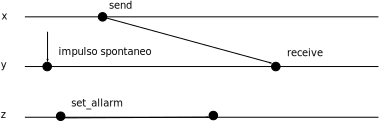
\includegraphics[scale=0.8]{capitoli/introduzione_ambiente-distribuito/imgs/n_07}
\end{center}

\begin{itemize}
    \item \textbf{Evento di ricezione}: Rappresentato da una freccia che va da x
          ad y.
    \item \textbf{Evento di ring dell'allarme (when)}: Rappresentata da una
          freccia dal punto t' al punto t''
    \item \textbf{Evento spontaneo}: rappresentato da una piccola freccia che
          indica il punto t nella linea temporale dell'entità $x$ in cui l'evento
          avviene
\end{itemize}

Per convenzione, l'inizio del protocollo è dato dall'istante in cui si verifica
il primo impulso spontaneo. Infatti $t=0$ corrisponde al momento in cui il primo
impulso spontaneo si verifica:
\begin{center}
    \texttt{eventi\_iniziali} $=\lbrace$ impulsi spontanei $\rbrace$
\end{center}
Ci possono essere degli eventi \textbf{contemporanei} per cui impostiamo delle
precedenze, come:
\begin{center}
    \texttt{spontaneously} $\geq$ \texttt{sveglia} $\geq$ \texttt{receiving}
\end{center}

\subsection{Stati e Configurazioni}
La memoria privata di ogni entità, oltre al comportamento, contiene un insieme
di registri, alcuni già inizializzati, altri da inizializzare durante
l'esecuzione.\\
Il contenuto di tutti i registri dell'entità $x$ e il valore della sua sveglia
$c_x$ all'istante $t$ costituiscono quello che viene chiamato lo stato interno
di $x$ in $t$ ed è indicato con $\sigma (x, t)$. Indichiamo con $\sum(t)$
l'insieme degli stati interni al tempo $t$ di tutte le entità. Gli stati interni
cambiano con il tempo e il verificarsi di eventi.\\
C'è un fatto importante sugli stati interni. Consideriamo due ambienti diversi,
$E_1$ ed $E_2$ , dove, per caso, lo stato interno di $x$ all'istante $t$ è lo
stesso. Quindi $x$ non può distinguere tra i due ambienti, cioè $x$ non è in
grado di dire se si trova nell'ambiente $E_1$ o $E_2$.\\
C'è una conseguenza importante. Consideriamo la situazione appena descritta:
all'istante $t$, lo stato interno di $x$ è lo stesso sia in $E_1$ che in $E_2$.
Supponiamo ora che, anche per caso, si verifichi esattamente lo stesso evento in
$x$ (ad esempio, la sveglia suona o lo stesso messaggio viene ricevuto dallo
stesso vicino). Quindi $x$ eseguirà esattamente la stessa azione in entrambi i
casi e il suo stato interno continuerà ad essere lo stesso in entrambe le
situazioni.

\begin{prop}
    Assumendo che lo stesso evento si verifica in $x \in  \xi$
    al tempo $t$ in due differenti esecuzioni, e siano $\sigma_1$ e $\sigma_2$ gli
    stati interni di $x$ quando ciò si verifica, allora se $\sigma_1 = \sigma_2$,
    il nuovo stato interno di $x$ sarà lo stesso in entrambe le esecuzioni.\\
    Un'entità non riesce a distinguere tra le esecuzioni.
\end{prop}

\begin{prop}
    Assumendo che lo stesso evento si verifica in $x$ e $y$ al
    tempo $t$ e siano $\sigma_1$ e $\sigma_2$ i rispettivi stati interni, allora
    se $\sigma_1 = \sigma_2$ lo stato interno di $x$ e $y$ sarà ancora lo stesso.
    Dall'esterno non riusciamo a distinguere tra le entità.
\end{prop}

Lo stato globale di un sistema si può rappresentare mediante la
\textbf{configurazione} della rete al tempo $t$:

\begin{center}
    \texttt{C(t) = $(\Sigma(t)$, \texttt{Future(t)})}
\end{center}

dove:

\begin{itemize}
    \item $\sum(t)$ specifica lo stato interno di tutte le entità a tempo $t$.
    \item \texttt{Future(t)} è l'insieme di tutti gli eventi che si verificheranno
          a tempo $t$. Quindi se $future(t) = 0$ significa che non si dovranno generare
          più eventi.
\end{itemize}

La configurazione iniziale $C(0)$ contiene non solo l'insieme iniziale degli
stati $(0)$ ma anche l'insieme $Future(0)$ degli impulsi spontanei. Gli ambienti
che differiscono solo nella loro configurazione iniziale verranno chiamati
istanze dello stesso sistema.\\
La configurazione $C(t)$ è come un'istantanea del sistema all'istante $t$.


\section{Definizione formale di un problema}
Un algoritmo distribuito è l'insieme di regole che definiscono i comportamenti
delle entità. Il motivo per cui potremmo aver bisogno di progettare i
comportamenti è consentire alle entità di risolvere un determinato problema,
eseguire un'attività definita o fornire un servizio richiesto. In generale, ci
verrà dato un problema e il nostro compito è progettare un insieme di regole che
risolveranno sempre il problema in un tempo finito.

\begin{definition}
    Un problema $P$ è definito dalla terna:
    \begin{eqnarray}
        P = P_{INIT}, P_{FINAL}, R
        \nonumber
    \end{eqnarray}
    dove:
    \begin{itemize}
        \item $P_{INIT}$ è un predicato che specifica le condizioni iniziali;
        \item $P_{FINAL}$ è un predicato che specifica le condizioni finali;
        \item $R$ è l'insieme delle restrizioni. \end{itemize}
\end{definition}

% \definition{ Un problema $P$ è definito dalla terna:
%   \begin{eqnarray}
%     P = P_{INIT}, P_{FINAL}, R
%     \nonumber
%   \end{eqnarray}
%   dove:
%   \begin{itemize}
%     \item $P_{INIT}$ è un predicato che specifica le condizioni iniziali;
%     \item $P_{FINAL}$ è un predicato che specifica le condizioni finali;
%     \item $R$ è l'insieme delle restrizioni. \end{itemize}}

\paragraph{Esempio Broadcast:}
\begin{itemize}
    \item $P_{INIT}$ = ``Solo un'entità ha l'informazione $I$ al tempo $t=0$'':
          \begin{center}
              $(\exists x \in \xi : \textrm{value}_t(x) = I) ~~ \wedge ~~ (\forall
                  y \neq x \in \xi,~\textrm{value}_t(y) = \emptyset)$
          \end{center}

          \texttt{Future(t)} = $i$ su $x$ ($i$ rappresenta l'impulso spontaneo
          su $x$).

    \item $P_{FINAL}$ = ``Tutte le entità hanno l'informazione $I$ al tempo
          $t$'':
          \begin{center}
              $\forall x \in \xi : \textrm{value}_t(x) = I$
          \end{center}

    \item $R$ = Affidabilità totale; connettività; link bidirezionali.
\end{itemize}

\subsection{Stati}
Sia $B$ un protocollo che da la soluzione al problema P=$<P_{init}, P_{final},
    R>$. Parte di definizione del protocollo deve essere svolta dalla definizione
degli insiemi degli stati.
\begin{itemize}
    \item $S_{INIT}$: stati iniziali di tutte le entità all'inizio del protocollo
          (es: initiator, idle);
    \item $S_{TERM}$: stati terminali, una volta che questi stati sono raggiunti
          non potranno mai essere cambiati dal protocollo (es: done);
    \item $S_{INTERMEDI}$: Stati ne finali ne iniziali.
\end{itemize}

Gli stati iniziali e terminali sono, a loro volta, divisi in:
\begin{itemize}
    \item $S_{START}\subseteq S_{INIT} \Rightarrow$ Stati che danno inizio al
          protocollo (quindi quelli che possono ricevere l'impulso spontaneo).
    \item $S_{FINAL}\subseteq S_{TERM} \Rightarrow$ Le entità in $S_{FINAL}$ non
          eseguono più azioni, ovvero processano solo $nil$. Le entità in questi stati
          non possono comunque cambiare stato, poichè questo insieme è incluso in quelli
          terminali $S_{TERM}$.
\end{itemize}

Quindi si avrà che $S: S_{INIT} \cup S_{TERM} \cup S_{INTERMEDI}$

\subsection{Terminazione}
Un protocollo $B$ termina se per tutte le configurazioni iniziali $C(0)$ che
soddisfano $P_{INIT}$ e per tutte le esecuzioni che partono da tali
configurazioni il predicato
\begin{center}
    $\texttt{Terminate(t)} \equiv (\{STATUS_t\} \subseteq S_{TERM} \; \wedge \;
        \texttt{Future(t)} = \emptyset) \;$ vale per qualche \; $t>0$,
\end{center}
cioè tutte le entità entrano in uno stato terminale dopo un tempo finito e tutti
gli eventi generati si sono verificati. Quindi se tutte le entità entrano in uno
stato terminale dopo un certo tempo finito $t$ e tutti gli eventi generati si
sono verificati.\\
Un'entità non è a conoscenza di quando la terminazione avviene, in generale
vorremmo che ogni entità conosca almeno la terminazione locale. Questa
situazione è chiamata \verb|Explicit_Termination| e si verifica quando il predicato

\begin{center}
    $\texttt{Explicit\_Terminate(t)} \equiv (\{STATUS_t\} \subseteq S_{FINAL}) \;$
    vale per qualche $t>0$
\end{center}
Quindi la terminazione esplicita avviene quando tutte le entità entrano in uno
stato finale dopo un tempo finito.

%\textbf{Mio Terminazione:} Un protocollo B termina se per tutte le
%configurazioni iniziali $C(0)$ che soddisfano $P_{init}$ dopo un tempo finito
%tutte le entità entrano in stato Terminale e non si verificheranno più eventi,
%poichè $future(t)$ è vuoto.\\
%\textbf{Mio Terminazione\_Esplicita:}  Vogliamo che tutte le entità siano a
%conoscenza ALMENO della terminazione locale, per far questo quindi viene
%utilizzato l'insieme degli stati $S_{FINAL}$. Questa accade quando lo stato di
%un'entità è incluso in quell'insieme.

\subsection{Correttezza}

\begin{definition}
    Un protocollo $B$ è \textbf{corretto} se per tutte le esecuzioni
    che partono da una configurazione iniziale che soddisfa $P_{INIT}$:

    \begin{center}
        $\exists t>0$ tale che vale $Correct(t)$ dove $Correct(t) \equiv \forall t'
            \geq t$ vale $P_{FINAL}(t')$,
    \end{center}

\end{definition}

dove $Correct(t) \equiv (\forall t' \ge t, P_{FINAL}(t)$); cioè, il predicato
finale alla fine vale e non cambia.

\subsection{Soluzione}
L'insieme di regole $B$ \textbf{risolve} il problema $P$ se termina sempre
correttamente sotto le restrizioni $R$. Dato che abbiamo due tipi di
terminazione, abbiamo anche due tipi di soluzione:
\begin{itemize}
    \item \texttt{Simple\_solution(B, P)} = $\exists t > 0 :$ \texttt{Correct(t)}
          $ ~~ \wedge ~~$ \texttt{Terminate(t)}\\
          Ovvero che il predicato simple solution vale sotto le restrizioni R per
          ogni esecuzione che inizia da una configurazione iniziale che soddisfa
          $P_{init}$.

    \item \texttt{Explicit\_solution(B, P)} = $\exists t > 0 :$
          \texttt{Correct(t)} $ ~~ \wedge ~~$ \texttt{Explicit\_Terminate(t)}\\
          Ovvero che il predicato explicit solution vale sotto le restrizioni R
          per ogni esecuzione che inizia da una configurazione iniziale che
          soddisfa $P_{init}$.
\end{itemize}

% -------------------------------------------